\documentclass[12pt,a4paper]{article}
\usepackage[utf8]{vietnam}
\usepackage{amsmath,amssymb}
\usepackage{tabularx}
\usepackage{tikz}
\usepackage{xcolor}
\usepackage[top=0.6cm, bottom=0.6cm, left=0.6cm, right=0.6cm]{geometry}
\usepackage[dethi]{ex_test}

\SAOPTN{widthSA=2.8,heightSA=0.62}
\setlength{\parskip}{0pt}

% Dòng kẻ chấm mờ chuẩn viết tay
\newcommand{\dongke}[1]{%
  \begingroup%
  \setlength{\parskip}{0pt}%
  \baselineskip=18.5pt%
  \vspace{1.0mm}%
  \foreach \i in {1,...,#1}{%
    \noindent{\color{gray!60}\dotfill}\par%
  }%
  \vspace{0.6mm}%
  \endgroup%
}

% Khu vực bài làm chia 2 cột có vách ngăn mờ ở giữa
\newcommand{\dongkeHaiCot}[1]{%
  \par\vspace{0.5mm}%
  \noindent%
  \begin{minipage}[t]{0.485\linewidth}%
    \dongke{#1}%
  \end{minipage}%
  \hfill%
  {\color{gray!60}\vrule}%
  \hfill%
  \begin{minipage}[t]{0.485\linewidth}%
    \dongke{#1}%
  \end{minipage}%
}

% Định nghĩa ô bài tập tự luận trong bảng
\newcommand{\oBaiTap}[3][5]{%
  \vspace{1.0mm}%
  \noindent\textbf{#2} #3\par%
  \dongke{#1}%
}

\begin{document}
\pagestyle{empty}
% =============================================================================
% ========================= MA DE 101 - MAT TRUOC (TRANG 1/2) =============
% =============================================================================
\noindent
\begin{tabularx}{\linewidth}{|X|c|}
\hline
\textbf{PHIẾU KIỂM TRA ĐỊNH KỲ TOÁN 8 - TUẦN 12 - BUỔI 01} & \textbf{Mã đề: 101 - Trang 1/2} \\
\hline
\end{tabularx}

\vspace{1.0mm}

\noindent
\begin{tabularx}{\linewidth}{|p{3.2cm}|X|}
\hline
\centering\textbf{ĐIỂM SỐ} & \centering\textbf{LỜI NHẬN XÉT CỦA THẦY CÔ} \tabularnewline
\hline
\rule{0pt}{1.8cm} & \tabularnewline
\hline
\end{tabularx}

\vspace{1.2mm}
\noindent\textbf{Câu 1 (0,25 điểm).} Cho $\Delta ABC$ vuông tại $A$ có $AB = 3\text{ cm}, AC = 4\text{ cm}$. Tính $BC =$ \shortans{5\text{ cm}}\par\vspace{1.5mm}
\noindent\textbf{Câu 2 (0,25 điểm).} Cho $\Delta ABC, MN \parallel BC$. Biết $AM = 2, AB = 6, BC = 9$. Tính $MN =$ \shortans{3}\par\vspace{1.5mm}
\noindent\textbf{Câu 3 (0,25 điểm).} Cho $\Delta ABC, DE \parallel BC$. Biết $AD = 2, DB = 4, AE = 3$. Tính $EC =$ \shortans{6}\par\vspace{1.5mm}
\noindent\textbf{Câu 4 (0,25 điểm).} Điều kiện xác định của phân thức $\dfrac{2x + 1}{x - 3}$ là: \shortans{x \ne 3}\par\vspace{1.5mm}
\noindent\textbf{Câu 5 (0,25 điểm).} Giá trị của phân thức $P = \dfrac{x + 2}{x - 1}$ tại $x = 3$ là: \shortans{\dfrac{5}{2}}\par\vspace{1.5mm}
\noindent\textbf{Câu 6 (0,25 điểm).} Rút gọn phân thức $\dfrac{6x^2y}{9xy^2} =$ (với $xy \ne 0$): \shortans{\dfrac{2x}{3y}}\par\vspace{1.5mm}
\noindent\textbf{Câu 7 (0,25 điểm).} Với giá trị nào của $x$ thì phân thức $\dfrac{2x - 6}{x + 1} = 0$? \shortans{x = 3}\par\vspace{1.5mm}
\noindent\textbf{Câu 8 (0,25 điểm).} Điền vào chỗ trống: $\dfrac{x - 1}{x + 2} = \dfrac{\dots}{x^2 - 4}$. \shortans{(x - 1)(x - 2)}\par\vspace{1.5mm}
\noindent\textbf{Câu 9 (0,25 điểm).} Cọc $1\text{ m}$ bóng $1{,}5\text{ m}$; cột cờ bóng $9\text{ m}$. Chiều cao cột cờ là: \shortans{6\text{ m}}\par\vspace{1.5mm}
\noindent\textbf{Câu 10 (0,25 điểm).} Rút gọn phân thức $\dfrac{x^2 - 25}{x - 5} =$ (với $x \ne 5$): \shortans{x + 5}\par\vspace{1.5mm}
\vspace{0.2mm}
\noindent\textbf{Câu 11 (3,0 điểm). Rút gọn các phân thức đại số sau:}
\vspace{0.5mm}

\noindent
\begin{tabularx}{\linewidth}{|X|X|}
\hline
\oBaiTap[5]{a) (0,5 điểm)}{$\dfrac{3x + 9}{x^2 - 9}$} & 
\oBaiTap[5]{b) (0,5 điểm)}{$\dfrac{x^2 - 16}{(x + 4)^2}$} \\
\hline
\oBaiTap[5]{c) (0,5 điểm)}{$\dfrac{x^2 - 6x + 9}{2x - 6}$} & 
\oBaiTap[5]{d) (0,5 điểm)}{$\dfrac{xy - 2y + 3x - 6}{x^2 - 4}$} \\
\hline
\oBaiTap[5]{e) (0,5 điểm)}{$\dfrac{x^2 - 3x}{x^2 - 9}$} & 
\oBaiTap[5]{f) (0,5 điểm)}{$\dfrac{x^2 - 4x + 4}{x^2 - 4}$} \\
\hline
\end{tabularx}

\newpage
% =============================================================================
% ========================= MA DE 101 - MAT SAU (TRANG 2/2) ==============
% =============================================================================
\noindent
\begin{tabularx}{\linewidth}{|X|}
\hline
\centering\textbf{TOÁN 8 - TUẦN 12 - BUỔI 01 | Mã đề: 101 - Trang 2/2} \\
\hline
\end{tabularx}

\vspace{2.2mm}

\noindent\textbf{Câu 12 (2,0 điểm). Tìm $x$, biết:}
\vspace{0.5mm}

\noindent
\begin{tabularx}{\linewidth}{|X|X|}
\hline
\oBaiTap[5]{a) (0,5 điểm)}{$\dfrac{2x - 1}{3} = \dfrac{x + 2}{2}$} & 
\oBaiTap[5]{b) (0,5 điểm)}{$(2x - 6)(x + 5) = 0$} \\
\hline
\oBaiTap[5]{c) (0,5 điểm)}{$\dfrac{x^2 - 9}{x - 3} = 0$} & 
\oBaiTap[5]{d) (0,5 điểm)}{$x^2 - 6x + 9 = 0$} \\
\hline
\end{tabularx}

\vspace{2.2mm}

\noindent
\begin{tabularx}{\linewidth}{|X|}
\hline
\vspace{0.5mm}
\begin{minipage}[t]{0.62\linewidth}
\vspace{0pt}
\textbf{Câu 13 (2,0 điểm).} Cho tam giác $ABC$ vuông tại $A$ có $AB = 6\text{ cm}, AC = 8\text{ cm}$.\par\vspace{0.3mm}
\textbf{a) (1,0 điểm)} Tính độ dài cạnh huyền $BC$.\par\vspace{0.3mm}
\textbf{b) (1,0 điểm)} Trên cạnh $AB$ lấy điểm $D$ sao cho $AD = 3\text{ cm}$. Kẻ đường thẳng qua $D$ song song với $BC$ cắt cạnh $AC$ tại $E$. Tính độ dài các đoạn thẳng $AE$ và $DE$.
\end{minipage}\hfill
\begin{minipage}[t]{0.36\linewidth}
\vspace{0pt}\centering
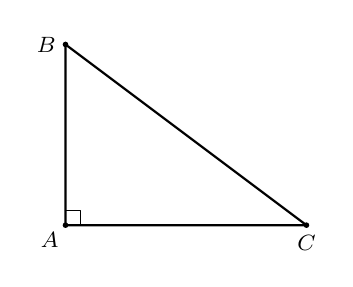
\begin{tikzpicture}[scale=0.85, >=stealth, line join=round, line cap=round, font=\footnotesize]
  \coordinate (A) at (0, 0);
  \coordinate (B) at (0, 2.7);
  \coordinate (C) at (3.6, 0);

  \draw[thick] (A) -- (B) -- (C) -- cycle;

  % Vuông góc tại A
  \draw (0, 0.22) -- (0.22, 0.22) -- (0.22, 0);

  \fill (A) circle (1.2pt) node[below left=-1pt] {$A$};
  \fill (B) circle (1.2pt) node[left] {$B$};
  \fill (C) circle (1.2pt) node[below] {$C$};
\end{tikzpicture}
\end{minipage}\par
\vspace{0.4mm}
\noindent\textit{Bài giải:}\dongkeHaiCot{10}
\\ \hline
\end{tabularx}

\vspace{2.2mm}

\noindent
\begin{tabularx}{\linewidth}{|X|}
\hline
\vspace{0.5mm}
\textbf{Câu 14 (0,5 điểm).} Tìm giá trị lớn nhất của biểu thức: $A = \dfrac{12}{x^2 - 4x + 7}$ với $x \in \mathbb{R}$.\par
\vspace{0.4mm}
\noindent\textit{Bài giải:}\dongkeHaiCot{6}
\\ \hline
\end{tabularx}

\newpage
% =============================================================================
% ========================= MA DE 102 - MAT TRUOC (TRANG 1/2) =============
% =============================================================================
\noindent
\begin{tabularx}{\linewidth}{|X|c|}
\hline
\textbf{PHIẾU KIỂM TRA ĐỊNH KỲ TOÁN 8 - TUẦN 12 - BUỔI 01} & \textbf{Mã đề: 102 - Trang 1/2} \\
\hline
\end{tabularx}

\vspace{1.0mm}

\noindent
\begin{tabularx}{\linewidth}{|p{3.2cm}|X|}
\hline
\centering\textbf{ĐIỂM SỐ} & \centering\textbf{LỜI NHẬN XÉT CỦA THẦY CÔ} \tabularnewline
\hline
\rule{0pt}{1.8cm} & \tabularnewline
\hline
\end{tabularx}

\vspace{1.2mm}
\noindent\textbf{Câu 1 (0,25 điểm).} Cho $\Delta ABC$ vuông tại $A$ có $AB = 6\text{ cm}, BC = 10\text{ cm}$. Tính $AC =$ \shortans{8\text{ cm}}\par\vspace{1.5mm}
\noindent\textbf{Câu 2 (0,25 điểm).} Cho $\Delta ABC, MN \parallel BC$. Biết $AM = 3, AB = 6, BC = 8$. Tính $MN =$ \shortans{4}\par\vspace{1.5mm}
\noindent\textbf{Câu 3 (0,25 điểm).} Cho $\Delta ABC, DE \parallel BC$. Biết $AD = 3, DB = 6, AE = 2$. Tính $EC =$ \shortans{4}\par\vspace{1.5mm}
\noindent\textbf{Câu 4 (0,25 điểm).} Điều kiện xác định của phân thức $\dfrac{3x - 2}{x - 5}$ là: \shortans{x \ne 5}\par\vspace{1.5mm}
\noindent\textbf{Câu 5 (0,25 điểm).} Giá trị của phân thức $P = \dfrac{x + 3}{x - 2}$ tại $x = 4$ là: \shortans{\dfrac{7}{2}}\par\vspace{1.5mm}
\noindent\textbf{Câu 6 (0,25 điểm).} Rút gọn phân thức $\dfrac{8x^3y}{12x^2y^2} =$ (với $xy \ne 0$): \shortans{\dfrac{2x}{3y}}\par\vspace{1.5mm}
\noindent\textbf{Câu 7 (0,25 điểm).} Với giá trị nào của $x$ thì phân thức $\dfrac{3x - 12}{x + 2} = 0$? \shortans{x = 4}\par\vspace{1.5mm}
\noindent\textbf{Câu 8 (0,25 điểm).} Điền vào chỗ trống: $\dfrac{x + 1}{x - 3} = \dfrac{\dots}{x^2 - 9}$. \shortans{(x + 1)(x + 3)}\par\vspace{1.5mm}
\noindent\textbf{Câu 9 (0,25 điểm).} Cọc $1\text{ m}$ bóng $1{,}2\text{ m}$; cột cờ bóng $6\text{ m}$. Chiều cao cột cờ là: \shortans{5\text{ m}}\par\vspace{1.5mm}
\noindent\textbf{Câu 10 (0,25 điểm).} Rút gọn phân thức $\dfrac{x^2 - 36}{x - 6} =$ (với $x \ne 6$): \shortans{x + 6}\par\vspace{1.5mm}
\vspace{0.2mm}
\noindent\textbf{Câu 11 (3,0 điểm). Rút gọn các phân thức đại số sau:}
\vspace{0.5mm}

\noindent
\begin{tabularx}{\linewidth}{|X|X|}
\hline
\oBaiTap[5]{a) (0,5 điểm)}{$\dfrac{4x + 12}{x^2 - 9}$} & 
\oBaiTap[5]{b) (0,5 điểm)}{$\dfrac{x^2 - 25}{(x + 5)^2}$} \\
\hline
\oBaiTap[5]{c) (0,5 điểm)}{$\dfrac{x^2 - 8x + 16}{3x - 12}$} & 
\oBaiTap[5]{d) (0,5 điểm)}{$\dfrac{xy - 3y + 2x - 6}{x^2 - 9}$} \\
\hline
\oBaiTap[5]{e) (0,5 điểm)}{$\dfrac{x^2 - 4x}{x^2 - 16}$} & 
\oBaiTap[5]{f) (0,5 điểm)}{$\dfrac{x^2 - 6x + 9}{x^2 - 9}$} \\
\hline
\end{tabularx}

\newpage
% =============================================================================
% ========================= MA DE 102 - MAT SAU (TRANG 2/2) ==============
% =============================================================================
\noindent
\begin{tabularx}{\linewidth}{|X|}
\hline
\centering\textbf{TOÁN 8 - TUẦN 12 - BUỔI 01 | Mã đề: 102 - Trang 2/2} \\
\hline
\end{tabularx}

\vspace{2.2mm}

\noindent\textbf{Câu 12 (2,0 điểm). Tìm $x$, biết:}
\vspace{0.5mm}

\noindent
\begin{tabularx}{\linewidth}{|X|X|}
\hline
\oBaiTap[5]{a) (0,5 điểm)}{$\dfrac{3x - 1}{4} = \dfrac{x + 3}{2}$} & 
\oBaiTap[5]{b) (0,5 điểm)}{$(3x - 9)(x + 4) = 0$} \\
\hline
\oBaiTap[5]{c) (0,5 điểm)}{$\dfrac{x^2 - 16}{x - 4} = 0$} & 
\oBaiTap[5]{d) (0,5 điểm)}{$x^2 - 8x + 16 = 0$} \\
\hline
\end{tabularx}

\vspace{2.2mm}

\noindent
\begin{tabularx}{\linewidth}{|X|}
\hline
\vspace{0.5mm}
\begin{minipage}[t]{0.62\linewidth}
\vspace{0pt}
\textbf{Câu 13 (2,0 điểm).} Cho tam giác $ABC$ vuông tại $A$ có $AB = 9\text{ cm}, AC = 12\text{ cm}$.\par\vspace{0.3mm}
\textbf{a) (1,0 điểm)} Tính độ dài cạnh huyền $BC$.\par\vspace{0.3mm}
\textbf{b) (1,0 điểm)} Trên cạnh $AB$ lấy điểm $D$ sao cho $AD = 6\text{ cm}$. Kẻ đường thẳng qua $D$ song song với $BC$ cắt cạnh $AC$ tại $E$. Tính độ dài các đoạn thẳng $AE$ và $DE$.
\end{minipage}\hfill
\begin{minipage}[t]{0.36\linewidth}
\vspace{0pt}\centering
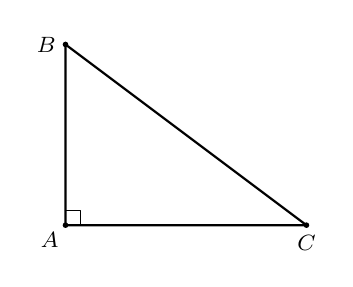
\begin{tikzpicture}[scale=0.85, >=stealth, line join=round, line cap=round, font=\footnotesize]
  \coordinate (A) at (0, 0);
  \coordinate (B) at (0, 2.7);
  \coordinate (C) at (3.6, 0);

  \draw[thick] (A) -- (B) -- (C) -- cycle;

  % Vuông góc tại A
  \draw (0, 0.22) -- (0.22, 0.22) -- (0.22, 0);

  \fill (A) circle (1.2pt) node[below left=-1pt] {$A$};
  \fill (B) circle (1.2pt) node[left] {$B$};
  \fill (C) circle (1.2pt) node[below] {$C$};
\end{tikzpicture}
\end{minipage}\par
\vspace{0.4mm}
\noindent\textit{Bài giải:}\dongkeHaiCot{10}
\\ \hline
\end{tabularx}

\vspace{2.2mm}

\noindent
\begin{tabularx}{\linewidth}{|X|}
\hline
\vspace{0.5mm}
\textbf{Câu 14 (0,5 điểm).} Tìm giá trị lớn nhất của biểu thức: $B = \dfrac{15}{x^2 - 6x + 14}$ với $x \in \mathbb{R}$.\par
\vspace{0.4mm}
\noindent\textit{Bài giải:}\dongkeHaiCot{6}
\\ \hline
\end{tabularx}

\newpage
% =============================================================================
% ========================= MA DE 103 - MAT TRUOC (TRANG 1/2) =============
% =============================================================================
\noindent
\begin{tabularx}{\linewidth}{|X|c|}
\hline
\textbf{PHIẾU KIỂM TRA ĐỊNH KỲ TOÁN 8 - TUẦN 12 - BUỔI 01} & \textbf{Mã đề: 103 - Trang 1/2} \\
\hline
\end{tabularx}

\vspace{1.0mm}

\noindent
\begin{tabularx}{\linewidth}{|p{3.2cm}|X|}
\hline
\centering\textbf{ĐIỂM SỐ} & \centering\textbf{LỜI NHẬN XÉT CỦA THẦY CÔ} \tabularnewline
\hline
\rule{0pt}{1.8cm} & \tabularnewline
\hline
\end{tabularx}

\vspace{1.2mm}
\noindent\textbf{Câu 1 (0,25 điểm).} Cho $\Delta ABC$ vuông tại $A$ có $AB = 5\text{ cm}, AC = 12\text{ cm}$. Tính $BC =$ \shortans{13\text{ cm}}\par\vspace{1.5mm}
\noindent\textbf{Câu 2 (0,25 điểm).} Cho $\Delta ABC, MN \parallel BC$. Biết $AM = 2, AB = 5, BC = 10$. Tính $MN =$ \shortans{4}\par\vspace{1.5mm}
\noindent\textbf{Câu 3 (0,25 điểm).} Cho $\Delta ABC, DE \parallel BC$. Biết $AD = 2, DB = 6, AE = 3$. Tính $EC =$ \shortans{9}\par\vspace{1.5mm}
\noindent\textbf{Câu 4 (0,25 điểm).} Điều kiện xác định của phân thức $\dfrac{x + 4}{x - 2}$ là: \shortans{x \ne 2}\par\vspace{1.5mm}
\noindent\textbf{Câu 5 (0,25 điểm).} Giá trị của phân thức $P = \dfrac{x + 1}{x - 3}$ tại $x = 5$ là: \shortans{3}\par\vspace{1.5mm}
\noindent\textbf{Câu 6 (0,25 điểm).} Rút gọn phân thức $\dfrac{10xy^3}{15x^2y^2} =$ (với $xy \ne 0$): \shortans{\dfrac{2y}{3x}}\par\vspace{1.5mm}
\noindent\textbf{Câu 7 (0,25 điểm).} Với giá trị nào của $x$ thì phân thức $\dfrac{4x - 8}{x + 3} = 0$? \shortans{x = 2}\par\vspace{1.5mm}
\noindent\textbf{Câu 8 (0,25 điểm).} Điền vào chỗ trống: $\dfrac{x - 2}{x + 1} = \dfrac{\dots}{x^2 - 1}$. \shortans{(x - 2)(x - 1)}\par\vspace{1.5mm}
\noindent\textbf{Câu 9 (0,25 điểm).} Cọc $2\text{ m}$ bóng $1{,}5\text{ m}$; cột cờ bóng $6\text{ m}$. Chiều cao cột cờ là: \shortans{8\text{ m}}\par\vspace{1.5mm}
\noindent\textbf{Câu 10 (0,25 điểm).} Rút gọn phân thức $\dfrac{x^2 - 49}{x - 7} =$ (với $x \ne 7$): \shortans{x + 7}\par\vspace{1.5mm}
\vspace{0.2mm}
\noindent\textbf{Câu 11 (3,0 điểm). Rút gọn các phân thức đại số sau:}
\vspace{0.5mm}

\noindent
\begin{tabularx}{\linewidth}{|X|X|}
\hline
\oBaiTap[5]{a) (0,5 điểm)}{$\dfrac{5x + 10}{x^2 - 4}$} & 
\oBaiTap[5]{b) (0,5 điểm)}{$\dfrac{x^2 - 36}{(x + 6)^2}$} \\
\hline
\oBaiTap[5]{c) (0,5 điểm)}{$\dfrac{x^2 - 4x + 4}{3x - 6}$} & 
\oBaiTap[5]{d) (0,5 điểm)}{$\dfrac{xy - 4y + 3x - 12}{x^2 - 16}$} \\
\hline
\oBaiTap[5]{e) (0,5 điểm)}{$\dfrac{x^2 - 5x}{x^2 - 25}$} & 
\oBaiTap[5]{f) (0,5 điểm)}{$\dfrac{x^2 - 8x + 16}{x^2 - 16}$} \\
\hline
\end{tabularx}

\newpage
% =============================================================================
% ========================= MA DE 103 - MAT SAU (TRANG 2/2) ==============
% =============================================================================
\noindent
\begin{tabularx}{\linewidth}{|X|}
\hline
\centering\textbf{TOÁN 8 - TUẦN 12 - BUỔI 01 | Mã đề: 103 - Trang 2/2} \\
\hline
\end{tabularx}

\vspace{2.2mm}

\noindent\textbf{Câu 12 (2,0 điểm). Tìm $x$, biết:}
\vspace{0.5mm}

\noindent
\begin{tabularx}{\linewidth}{|X|X|}
\hline
\oBaiTap[5]{a) (0,5 điểm)}{$\dfrac{2x + 1}{5} = \dfrac{x - 1}{2}$} & 
\oBaiTap[5]{b) (0,5 điểm)}{$(2x - 8)(x + 3) = 0$} \\
\hline
\oBaiTap[5]{c) (0,5 điểm)}{$\dfrac{x^2 - 25}{x - 5} = 0$} & 
\oBaiTap[5]{d) (0,5 điểm)}{$x^2 - 4x + 4 = 0$} \\
\hline
\end{tabularx}

\vspace{2.2mm}

\noindent
\begin{tabularx}{\linewidth}{|X|}
\hline
\vspace{0.5mm}
\begin{minipage}[t]{0.62\linewidth}
\vspace{0pt}
\textbf{Câu 13 (2,0 điểm).} Cho tam giác $ABC$ vuông tại $A$ có $AB = 8\text{ cm}, AC = 6\text{ cm}$.\par\vspace{0.3mm}
\textbf{a) (1,0 điểm)} Tính độ dài cạnh huyền $BC$.\par\vspace{0.3mm}
\textbf{b) (1,0 điểm)} Trên cạnh $AB$ lấy điểm $D$ sao cho $AD = 4\text{ cm}$. Kẻ đường thẳng qua $D$ song song với $BC$ cắt cạnh $AC$ tại $E$. Tính độ dài các đoạn thẳng $AE$ và $DE$.
\end{minipage}\hfill
\begin{minipage}[t]{0.36\linewidth}
\vspace{0pt}\centering
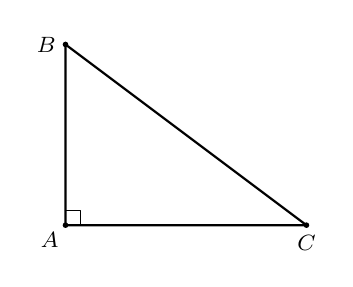
\begin{tikzpicture}[scale=0.85, >=stealth, line join=round, line cap=round, font=\footnotesize]
  \coordinate (A) at (0, 0);
  \coordinate (B) at (0, 2.7);
  \coordinate (C) at (3.6, 0);

  \draw[thick] (A) -- (B) -- (C) -- cycle;

  % Vuông góc tại A
  \draw (0, 0.22) -- (0.22, 0.22) -- (0.22, 0);

  \fill (A) circle (1.2pt) node[below left=-1pt] {$A$};
  \fill (B) circle (1.2pt) node[left] {$B$};
  \fill (C) circle (1.2pt) node[below] {$C$};
\end{tikzpicture}
\end{minipage}\par
\vspace{0.4mm}
\noindent\textit{Bài giải:}\dongkeHaiCot{10}
\\ \hline
\end{tabularx}

\vspace{2.2mm}

\noindent
\begin{tabularx}{\linewidth}{|X|}
\hline
\vspace{0.5mm}
\textbf{Câu 14 (0,5 điểm).} Tìm giá trị lớn nhất của biểu thức: $C = \dfrac{18}{x^2 - 2x + 7}$ với $x \in \mathbb{R}$.\par
\vspace{0.4mm}
\noindent\textit{Bài giải:}\dongkeHaiCot{6}
\\ \hline
\end{tabularx}

\newpage
% =============================================================================
% ========================= MA DE 104 - MAT TRUOC (TRANG 1/2) =============
% =============================================================================
\noindent
\begin{tabularx}{\linewidth}{|X|c|}
\hline
\textbf{PHIẾU KIỂM TRA ĐỊNH KỲ TOÁN 8 - TUẦN 12 - BUỔI 01} & \textbf{Mã đề: 104 - Trang 1/2} \\
\hline
\end{tabularx}

\vspace{1.0mm}

\noindent
\begin{tabularx}{\linewidth}{|p{3.2cm}|X|}
\hline
\centering\textbf{ĐIỂM SỐ} & \centering\textbf{LỜI NHẬN XÉT CỦA THẦY CÔ} \tabularnewline
\hline
\rule{0pt}{1.8cm} & \tabularnewline
\hline
\end{tabularx}

\vspace{1.2mm}
\noindent\textbf{Câu 1 (0,25 điểm).} Cho $\Delta ABC$ vuông tại $A$ có $AC = 12\text{ cm}, BC = 15\text{ cm}$. Tính $AB =$ \shortans{9\text{ cm}}\par\vspace{1.5mm}
\noindent\textbf{Câu 2 (0,25 điểm).} Cho $\Delta ABC, MN \parallel BC$. Biết $AM = 4, AB = 8, BC = 10$. Tính $MN =$ \shortans{5}\par\vspace{1.5mm}
\noindent\textbf{Câu 3 (0,25 điểm).} Cho $\Delta ABC, DE \parallel BC$. Biết $AD = 4, DB = 8, AE = 3$. Tính $EC =$ \shortans{6}\par\vspace{1.5mm}
\noindent\textbf{Câu 4 (0,25 điểm).} Điều kiện xác định của phân thức $\dfrac{5x + 1}{x - 4}$ là: \shortans{x \ne 4}\par\vspace{1.5mm}
\noindent\textbf{Câu 5 (0,25 điểm).} Giá trị của phân thức $P = \dfrac{x + 4}{x - 1}$ tại $x = 2$ là: \shortans{6}\par\vspace{1.5mm}
\noindent\textbf{Câu 6 (0,25 điểm).} Rút gọn phân thức $\dfrac{12x^2y^2}{18xy^3} =$ (với $xy \ne 0$): \shortans{\dfrac{2x}{3y}}\par\vspace{1.5mm}
\noindent\textbf{Câu 7 (0,25 điểm).} Với giá trị nào của $x$ thì phân thức $\dfrac{5x - 15}{x + 4} = 0$? \shortans{x = 3}\par\vspace{1.5mm}
\noindent\textbf{Câu 8 (0,25 điểm).} Điền vào chỗ trống: $\dfrac{x + 2}{x - 4} = \dfrac{\dots}{x^2 - 16}$. \shortans{(x + 2)(x + 4)}\par\vspace{1.5mm}
\noindent\textbf{Câu 9 (0,25 điểm).} Cọc $1\text{ m}$ bóng $1{,}5\text{ m}$; cột cờ bóng $12\text{ m}$. Chiều cao cột cờ là: \shortans{8\text{ m}}\par\vspace{1.5mm}
\noindent\textbf{Câu 10 (0,25 điểm).} Rút gọn phân thức $\dfrac{x^2 - 64}{x - 8} =$ (với $x \ne 8$): \shortans{x + 8}\par\vspace{1.5mm}
\vspace{0.2mm}
\noindent\textbf{Câu 11 (3,0 điểm). Rút gọn các phân thức đại số sau:}
\vspace{0.5mm}

\noindent
\begin{tabularx}{\linewidth}{|X|X|}
\hline
\oBaiTap[5]{a) (0,5 điểm)}{$\dfrac{2x + 8}{x^2 - 16}$} & 
\oBaiTap[5]{b) (0,5 điểm)}{$\dfrac{x^2 - 49}{(x + 7)^2}$} \\
\hline
\oBaiTap[5]{c) (0,5 điểm)}{$\dfrac{x^2 - 10x + 25}{2x - 10}$} & 
\oBaiTap[5]{d) (0,5 điểm)}{$\dfrac{xy - 5y + 2x - 10}{x^2 - 25}$} \\
\hline
\oBaiTap[5]{e) (0,5 điểm)}{$\dfrac{x^2 - 6x}{x^2 - 36}$} & 
\oBaiTap[5]{f) (0,5 điểm)}{$\dfrac{x^2 - 10x + 25}{x^2 - 25}$} \\
\hline
\end{tabularx}

\newpage
% =============================================================================
% ========================= MA DE 104 - MAT SAU (TRANG 2/2) ==============
% =============================================================================
\noindent
\begin{tabularx}{\linewidth}{|X|}
\hline
\centering\textbf{TOÁN 8 - TUẦN 12 - BUỔI 01 | Mã đề: 104 - Trang 2/2} \\
\hline
\end{tabularx}

\vspace{2.2mm}

\noindent\textbf{Câu 12 (2,0 điểm). Tìm $x$, biết:}
\vspace{0.5mm}

\noindent
\begin{tabularx}{\linewidth}{|X|X|}
\hline
\oBaiTap[5]{a) (0,5 điểm)}{$\dfrac{3x + 2}{5} = \dfrac{x + 2}{2}$} & 
\oBaiTap[5]{b) (0,5 điểm)}{$(3x - 12)(x + 2) = 0$} \\
\hline
\oBaiTap[5]{c) (0,5 điểm)}{$\dfrac{x^2 - 36}{x - 6} = 0$} & 
\oBaiTap[5]{d) (0,5 điểm)}{$x^2 - 10x + 25 = 0$} \\
\hline
\end{tabularx}

\vspace{2.2mm}

\noindent
\begin{tabularx}{\linewidth}{|X|}
\hline
\vspace{0.5mm}
\begin{minipage}[t]{0.62\linewidth}
\vspace{0pt}
\textbf{Câu 13 (2,0 điểm).} Cho tam giác $ABC$ vuông tại $A$ có $AB = 12\text{ cm}, AC = 9\text{ cm}$.\par\vspace{0.3mm}
\textbf{a) (1,0 điểm)} Tính độ dài cạnh huyền $BC$.\par\vspace{0.3mm}
\textbf{b) (1,0 điểm)} Trên cạnh $AB$ lấy điểm $D$ sao cho $AD = 4\text{ cm}$. Kẻ đường thẳng qua $D$ song song với $BC$ cắt cạnh $AC$ tại $E$. Tính độ dài các đoạn thẳng $AE$ và $DE$.
\end{minipage}\hfill
\begin{minipage}[t]{0.36\linewidth}
\vspace{0pt}\centering
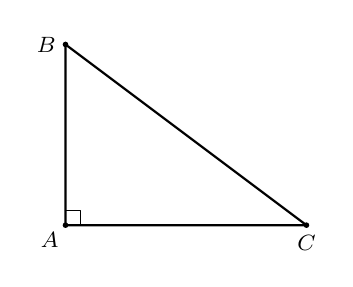
\begin{tikzpicture}[scale=0.85, >=stealth, line join=round, line cap=round, font=\footnotesize]
  \coordinate (A) at (0, 0);
  \coordinate (B) at (0, 2.7);
  \coordinate (C) at (3.6, 0);

  \draw[thick] (A) -- (B) -- (C) -- cycle;

  % Vuông góc tại A
  \draw (0, 0.22) -- (0.22, 0.22) -- (0.22, 0);

  \fill (A) circle (1.2pt) node[below left=-1pt] {$A$};
  \fill (B) circle (1.2pt) node[left] {$B$};
  \fill (C) circle (1.2pt) node[below] {$C$};
\end{tikzpicture}
\end{minipage}\par
\vspace{0.4mm}
\noindent\textit{Bài giải:}\dongkeHaiCot{10}
\\ \hline
\end{tabularx}

\vspace{2.2mm}

\noindent
\begin{tabularx}{\linewidth}{|X|}
\hline
\vspace{0.5mm}
\textbf{Câu 14 (0,5 điểm).} Tìm giá trị lớn nhất của biểu thức: $D = \dfrac{20}{x^2 - 8x + 20}$ với $x \in \mathbb{R}$.\par
\vspace{0.4mm}
\noindent\textit{Bài giải:}\dongkeHaiCot{6}
\\ \hline
\end{tabularx}
\end{document}
